% This is "sig-alternate.tex" V2.1 April 2013
% This file should be compiled with V2.5 of "sig-alternate.cls" May 2012
%
% This example file demonstrates the use of the 'sig-alternate.cls'
% V2.5 LaTeX2e document class file. It is for those submitting
% articles to ACM Conference Proceedings WHO DO NOT WISH TO
% STRICTLY ADHERE TO THE SIGS (PUBS-BOARD-ENDORSED) STYLE.
% The 'sig-alternate.cls' file will produce a similar-looking,
% albeit, 'tighter' paper resulting in, invariably, fewer pages.
%
% ----------------------------------------------------------------------------------------------------------------
% This .tex file (and associated .cls V2.5) produces:
%       1) The Permission Statement
%       2) The Conference (location) Info information
%       3) The Copyright Line with ACM data
%       4) NO page numbers
%
% as against the acm_proc_article-sp.cls file which
% DOES NOT produce 1) thru' 3) above.
%
% Using 'sig-alternate.cls' you have control, however, from within
% the source .tex file, over both the CopyrightYear
% (defaulted to 200X) and the ACM Copyright Data
% (defaulted to X-XXXXX-XX-X/XX/XX).
% e.g.
% \CopyrightYear{2007} will cause 2007 to appear in the copyright line.
% \crdata{0-12345-67-8/90/12} will cause 0-12345-67-8/90/12 to appear in the copyright line.
%
% ---------------------------------------------------------------------------------------------------------------
% This .tex source is an example which *does* use
% the .bib file (from which the .bbl file % is produced).
% REMEMBER HOWEVER: After having produced the .bbl file,
% and prior to final submission, you *NEED* to 'insert'
% your .bbl file into your source .tex file so as to provide
% ONE 'self-contained' source file.
%
% ================= IF YOU HAVE QUESTIONS =======================
% Questions regarding the SIGS styles, SIGS policies and
% procedures, Conferences etc. should be sent to
% Adrienne Griscti (griscti@acm.org)
%
% Technical questions _only_ to
% Gerald Murray (murray@hq.acm.org)
% ===============================================================
%
% For tracking purposes - this is V2.0 - May 2012

\documentclass{sig-alternate-05-2015}

\usepackage{graphicx}
\usepackage{caption}
\usepackage{subcaption}

\usepackage{amssymb}
\usepackage[T1]{fontenc}
\usepackage{bbm}
%\usepackage{amsthm}
\usepackage[utf8]{inputenc}
\usepackage{lipsum}
\usepackage{graphicx}
\usepackage[caption=false]{subfig}
\usepackage{graphicx}
\usepackage{csvsimple}
%\usepackage{array}
\usepackage{float}
\usepackage{amsmath}
\usepackage{pgfplotstable}
%\usepackage[demo]{graphicx}
%\usepackage{subcaption}
\usepackage{algorithm}
\usepackage[noend]{algpseudocode}
\usepackage{varwidth}

\newtheorem{lemma}{Lemma}
\newtheorem{definition}{Definition}
\newtheorem{remark}{Remark}
\newtheorem{corollary}{Corollary}

\begin{document}
\nocite{*}
% Copyright
\setcopyright{acmcopyright}
%\setcopyright{acmlicensed}
%\setcopyright{rightsretained}
%\setcopyright{usgov}
%\setcopyright{usgovmixed}
%\setcopyright{cagov}
%\setcopyright{cagovmixed}


% DOI
\doi{10.475/123_4}

% ISBN
\isbn{123-4567-24-567/08/06}

%Conference
\conferenceinfo{PLDI '13}{June 16--19, 2013, Seattle, WA, USA}

\acmPrice{\$15.00}

%
% --- Author Metadata here ---
\conferenceinfo{WOODSTOCK}{'97 El Paso, Texas USA}
%\CopyrightYear{2007} % Allows default copyright year (20XX) to be over-ridden - IF NEED BE.
%\crdata{0-12345-67-8/90/01}  % Allows default copyright data (0-89791-88-6/97/05) to be over-ridden - IF NEED BE.
% --- End of Author Metadata ---
\title{LDA Model Monitoring in Distributed Systems\titlenote{(Produces the permission block, and
copyright information). For use with
SIG-ALTERNATE.CLS. Supported by ACM.}}
\subtitle{[Extended Abstract]
\titlenote{A full version of this paper is available as
\textit{Author's Guide to Preparing ACM SIG Proceedings Using
\LaTeX$2_\epsilon$\ and BibTeX} at
\texttt{www.acm.org/eaddress.htm}}}
%
% You need the command \numberofauthors to handle the 'placement
% and alignment' of the authors beneath the title.
%
% For aesthetic reasons, we recommend 'three authors at a time'
% i.e. three 'name/affiliation blocks' be placed beneath the title.
%
% NOTE: You are NOT restricted in how many 'rows' of
% "name/affiliations" may appear. We just ask that you restrict
% the number of 'columns' to three.
%
% Because of the available 'opening page real-estate'
% we ask you to refrain from putting more than six authors
% (two rows with three columns) beneath the article title.
% More than six makes the first-page appear very cluttered indeed.
%
% Use the \alignauthor commands to handle the names
% and affiliations for an 'aesthetic maximum' of six authors.
% Add names, affiliations, addresses for
% the seventh etc. author(s) as the argument for the
% \additionalauthors command.
% These 'additional authors' will be output/set for you
% without further effort on your part as the last section in
% the body of your article BEFORE References or any Appendices.

\numberofauthors{4} %  in this sample file, there are a *total*
% of EIGHT authors. SIX appear on the 'first-page' (for formatting
% reasons) and the remaining two appear in the \additionalauthors section.
%
\author{
% You can go ahead and credit any number of authors here,
% e.g. one 'row of three' or two rows (consisting of one row of three
% and a second row of one, two or three).
%
% The command \alignauthor (no curly braces needed) should
% precede each author name, affiliation/snail-mail address and
% e-mail address. Additionally, tag each line of
% affiliation/address with \affaddr, and tag the
% e-mail address with \email.
%
% 1st. author
\alignauthor
Ran Bernstein\\
       \affaddr{Technion -- Israel Institute of Technology}\\
       \affaddr{Haifa 32000 Israel}\\
       \email{bernstein.ran@Gmail.com}
% 2nd. author
\alignauthor
 Daniel Keren\\
       \affaddr{University of Haifa}\\
       \affaddr{Haifa 31905 Israel}\\
       \email{dkeren@cs.haifa.ac.il}
% 3rd. author
\alignauthor
Margarita Osadchy\\
       \affaddr{University of Haifa}\\
       \affaddr{Haifa 31905 Israel}\\
       \email{rita@cs.haifa.ac.il }
\and  % use '\and' if you need 'another row' of author names
% 4th. author
\alignauthor Assaf Schuster\\
       \affaddr{Technion -- Israel Institute of Technology}\\
       \affaddr{Haifa 32000 Israel}\\
       \email{assaf@cs.technion.ac.il}
}
% There's nothing stopping you putting the seventh, eighth, etc.
% author on the opening page (as the 'third row') but we ask,
% for aesthetic reasons that you place these 'additional authors'
% in the \additional authors block, viz.

% Just remember to make sure that the TOTAL number of authors
% is the number that will appear on the first page PLUS the
% number that will appear in the \additionalauthors section.

\maketitle
\begin{abstract}
Real systems for mining dynamic data streams should be able to detect changes that affect the
accuracy of the global model. Most previous work addressed the centralized settings
and proposed solutions that were based on the statistics of error rates in the data stream.
In this work, we focus on distributed settings.
Model training in a distributed environment
requires centralizing the data from all nodes (synchronization), which is very
costly in term of communication.
In order to minimize the communication, a monitoring algorithm should be executed locally at each node,
while preserving the validity of the global model.
We propose the first communication-efficient algorithm for monitoring a classification model over
distributed, dynamic data streams. Linear Discriminant Analysis (LDA) is a popular algorithm
used for classification and dimensionality reduction in many fields and thus we chose it as our
classification model.
Our algorithm has strong theoretical guarantees of correctness and it is shown empirically to
reduce communication volume by up to two orders of magnitude (compared to synchronization in every round) on three real data sets from different worlds of content.
Moreover, our approach monitors the classification model itself as opposed
to its errors, which make it possible to detect the change before the error occurs and provide privacy of the local data.
\end{abstract}


%
% The code below should be generated by the tool at
% http://dl.acm.org/ccs.cfm
% Please copy and paste the code instead of the example below.
%
\begin{CCSXML}
<ccs2012>
<concept>
<concept_id>10002951.10003317.10003347.10003356</concept_id>
<concept_desc>Information systems~Clustering and classification</concept_desc>
<concept_significance>300</concept_significance>
</concept>
<concept>
<concept_id>10003752.10003809.10010172</concept_id>
<concept_desc>Theory of computation~Distributed algorithms</concept_desc>
<concept_significance>300</concept_significance>
</concept>
</ccs2012>
\end{CCSXML}

\ccsdesc[300]{Information systems~Clustering and classification}
\ccsdesc[300]{Theory of computation~Distributed algorithms}


%
% End generated code
%

%
%  Use this command to print the description
%
\printccsdesc

% We no longer use \terms command
%\terms{Theory}

\keywords{Linear Discriminant Analysis; Distributed Monitoring}

\section{Introduction}
In this work, we address the problem of mining data streams when the streaming data is
{\em distributed} over a large number of nodes.
We assume that the data generation process and the prediction problem are the same for all nodes.
However, the streaming data is not stationary; notably, it can change over time.
The change could be caused by a system fault (e.g., sensor failure) or by a transition
in the target concept.
Classic examples of real-life prediction problems that involve target
concept change are user preference prediction and fraud detection.
In the former, the choices of the user can change over time; in the latter, the fraudulent
transactions change constantly to avoid detection.
In both, the target concept changes over time, and if not detected, renders the prediction model inadequate.

Methods that detect changes in data over time are referred to as {\em concept drift detection} or {\em change-point detection}.
A large volume of work has been done on these topics
(see e.g., ~\cite{basseville1993detection,brodsky2013nonparametric,ChenGupta2000,Tsymbal,Gama2014}
for in-depth surveys of the field).
The solutions, proposed in previous work cover different forms of data change:
the input data characteristics, or the relation between the input data and the target variable, or both.
Some forms of change will influence the prediction model and some will not
(even though the second kind could be detected as a change in the distribution underlying the data and
might mistakenly indicate that a re-computation of the prediction model is required.).
In this work, we are only concerned with the changes that affect the model.
Our method is distinct from the previous work in the following important aspects:

\begin{description}
\item[Model-Based Monitoring] We focus on monitoring a classification model.
Most previous work on concept drift detection~\cite{baena2006early,gama2004learning,Nishida2007},
concerned with classification, is error-based  (utilizing classification error rates to
draw conclusions about the change in the distribution).
Here, we propose to monitor the change in the {\em model} itself as opposed to errors in classification.
Monitoring the model and not the errors has an important benefit: the drift can
be detected before the prediction error occurs.

\item[Distributed Setting]
    Concept drift has been actively studied in centralized settings.
    Our is one of the very few works \cite{AngGZPH13} that detects concept drift in a distributed
    environment, which is a critical part of a real big data system.
    In such systems, data is distributed over a large number of nodes and the model is learned
    globally, after the data is centralized from all the nodes (hereafter, synchronization).
    This process requires a lot of resources and communication.
    Thus it is crucial to minimize the number of synchronisations.
    Our approach for monitoring the global model over a distributed system
    provides provable guarantees of correctness, while existing methods for detection of concept
    drift in distributed settings~\cite{AngGZPH13} rely on heuristics, utilizing error rate statistics.

\item[Data Privacy]
    One of the important aspects in distributed systems is privacy of the data, 
    namely, each node does not learn the data of other nodes. 
    For example, nodes correspond to different hospitals that are not allowed 
    to share patient information with each other, but want to perform 
    collaborative training to improve the global model (using a trusted third party). 
    Methods that analyse classification errors to detect the concept drift, 
    require knowledge of the global model. If the goal is to protect the 
    privacy of the data in local nodes from each other, then the information, 
    received by the local nodes should not reveal private information from other 
    nodes (either directly or indirectly by learning private information from the 
    parameters of the model). 
    In our method, we monitor the correctness of the global model without 
    reveling the model to the nodes. The global information that is required 
    for our algorithm is the global covariance matrix of the feature space 
    and the norm of the model. These are not enough to recover the global model, 
    as the global means of the classes are not presented to the local nodes 
    while LDA needs class means to compute the classification model.
\end{description}

Similarly to~\cite{icml2014c2_harel14}, we link the concept drift detection method with the
hypothesis class and the training algorithm.
In this paper we focus on linear binary classifiers as a hypothesis class, and
LDA \cite{fisher1936use} as the learning algorithm.
We focus on linear classifiers, as they are well studied, allowing a solid platform for analyzing new concepts. Linear classifiers are also very popular in real applications and serve as a platform for more complex classifiers, such as ensemble models~\cite{Deva, eSVM},
neural networks~\cite{osadchy2015k}, and even deep architectures\cite{ROSS}.


\subsection{Our Contribution}
We propose Distributed Linear Discriminant Analysis
\\ (DLDA): a novel communication-efficient algorithm for monitoring LDA classifier over a distributed, dynamic data streams.
The proposed approach monitors the model itself, rather than classification errors,
and detects concept drift in streaming data, before the errors occur and preserves privacy of the data.
The algorithm provides strong theoretical guarantees of correctness.
We show empirically on three real data sets of different size and world of content that the proposed
method reduces communication to a fraction than synchronizing every round.


\section{Related Work}
Monitoring dynamic data streams is a broad topic that has been addressed in different research communities. Within this field, we focus on detecting a change in the data stream that renders the prediction model invalid. This problem is similar to concept drift detection, which was actively studied in centralized settings~\cite{basseville1993detection,brodsky2013nonparametric,ChenGupta2000,Tsymbal,Gama2014}.

Among methods for concept drift in classification are e.g., \cite{gama2004learning,baena2006early,klinkenberg2000detecting,dries2009adaptive,icml2014c2_harel14,AngGZPH13}. Drift Detection Method (DDM) \cite{gama2004learning} is one of the most widely used algorithm and it analyses the sum of overall classification error and its empirical standard deviation to detect the concept drift.
The Early Drift Detection Method (EDDM) \cite{baena2006early} achieves better detection results than DDM if the data stream changes gradually. EDDM monitors the distance between the two classification errors.
Linear Four Rates (LFR) \cite{wang2015concept} uses as a statistic a linear combination of all history errors, with a decay parameter. The approach specified in \cite{klinkenberg2000detecting,dries2009adaptive} makes use of
the SVM error for detection. All these solutions are based on analysis of classification error, hence they detect the drift only after the model becomes inaccurate.

In distributed settings, the problem of detecting a change in the data stream is referred to as {\em distributed monitoring}, and it is concerned with designing local tests for monitoring a function, defined globally over all the nodes in the system.
In this work, we focus on monitoring a global classification model, namely LDA, over distributed data.
We aim to define a constraint over the local data (at each node) that guarantees the validity of the global model. If a local data (in one or more nodes) does not meet the local condition, it leads to synchronization, i.e., the local data is collected to a central location from all the nodes and the model is recomputed.
The synchronization process has large communication costs, and the goal of the distributed monitoring methods is thus to minimize the number of synchronizations.

Most of the work in distributed monitoring has been concerned with simple 
functions of the data, such as 
linear~\cite{keralapura2006communication, kashyap2008efficient} or 
monotonic \cite{michel2005klee} functions. 
For non-linear functions, examples include work on monitoring the value 
of a single-variable polynomial~\cite{shah2008handling}, 
and eigenvalue perturbation~\cite{huang2007communication}. 
A generic geometric approach for monitoring arbitrary functions was proposed 
in~\cite{sharfman2007geometric}, and later extended and generalized 
in~\cite{keren2012shape,lazerson2015monitoring}.

A recently introduced work on monitoring Least Square 
Regression (LSR) ~\cite{gabel2015monitoring} is the closest to ours, 
but unlike the global scatter matrix (that is required by LSR) the global
covariance matrix (that is required in LDA) is not the mean of the 
local covariance matrices, things that complicated the theoretical framework. 


\section{Theoretical Foundation}
We first describe the Linear Discriminant Analysis (LDA) algorithm. 
We then define the monitoring problem and introduce our solution to it 
using convex set constraints.

\subsection{Linear Discriminant Analysis}%\\ \par
LDA seeks for a linear combination of features that characterize or separate two or more classes of samples.
The resulting combination may be used as a linear classifier, or for dimensionality reduction before later classification.

In LDA the problem is approached by assuming that the conditional probability
density functions $P(\vec x|y=p)$ and $P(\vec x|y=q)$ are both normally distributed with
mean and covariance parameters $\left(\vec \mu_p, B_p\right)$ and
$\left(\vec \mu_q, B_q\right)$, for two target classes p and q respectively.
${(x_1,y_1),\ldots,(x_n,y_n)}$ are i.i.d. samples, $x_i \in \mathbb{R}^d$
and $y_i \in \{0,1\}$.

% Let ${(x_1,y_1),\ldots,(x_n,y_n)}$ be a set of n observation pairs of $d < n$
% independent variables and one dependent variable, where $x_i$ are column vectors in $\mathbb{R}^d$, and $y_i$ are the
% corresponding classes.
We seek a linear transformation (model), $w \in \mathbb{R}^d $,
that maximizes the separation between the classes, where the separation is
defined to be the ratio of the variance between the classes to the variance
within the classes:
\begin{equation*}
S := \frac{\sigma^2_{between}}{\sigma^2_{within}} = \frac{(w^T (\mu_p -
\mu_q))^2}{w^T(B_p+B_q)w}.
\end{equation*}
Under this assumption, the Bayes optimal decision criterion is a threshold on the
dot product
\begin{equation*} \label{eq:decision}
w \cdot x > c
\end{equation*}
for some threshold constant c, where
\begin{equation} \label{eq:w}
w \propto (B_p+B_q)^{-1}(\mu_p - \mu_q)
\end{equation}
\begin{equation} \label{eq:c}
c = \frac{1}{2}(T-{\mu_p}^T S_p^{-1} {\mu_p}+{\mu_q}^T S_q^{-1} {\mu_q}).
\end{equation}
In this work we monitor $w$, and will refer it as the
classification \textit{model}.

\subsection{Problem Definition}
We denote $k$ as the number of nodes and
$n$ as the number of samples in a node.
Our model use discrete time (hereafter, rounds). Every node receives a new sample
in a round.
We use the \textit{sliding window} model where every node computes its current
parameters from the last $W$ samples it saw.
Every node keeps two sliding windows (one for each class) of length of $W/2$, as
a node receive a new observation it replaces the oldest one from its class.
$x^i_j$ and $y^i_j$ are the $j$'th sample and label in the $i$'th node
and $x_{old}^i(p)$ and $x_{old}^i(q)$ are the oldest samples from each class in
the sliding window of the $i$'th node. 
As data evolves, it is possible that the previously computed model
no longer matches the current true model.
Let $w_0$ be the existing model (vector of weights of a linear classifier),
previously computed at some point in the past (the synchronization time),
and let $w$ be the true
(The true model is the one we would obtained if we had aggregated the current observations
from all of the nodes into one place and computed the model according to it) LDA
model.
We wish to maintain an accurate estimation $w_0$ of the current global LDA model, $w$.
The question is then when to update the model.
Given an error threshold $T$, our goal is to raise an alert if
\begin{equation} \label{eq:coneCritiria}
\frac{<w,w_0>}{\parallel w \parallel \parallel w_0 \parallel}  < T.
\end{equation}
Due to the complexity of Eq. \ref{eq:coneCritiria},
we will monitor a simpler problem whose solution also satisfies
Eq. \ref{eq:coneCritiria}: the maximal volume sphere of which $w_0$ is its center
that resides completely inside the cone from Eq. ~\ref{eq:coneCritiria}.
This sphere is defined by
\begin{equation} \label{eq:critiria}
\parallel w-w_0 \parallel \  >  R_0,
\end{equation}
where $R_0 := \  \parallel w_0 \parallel \sqrt{1-T^2}$ is its radius.
Empirical evaluation showed that the values of 
$1-\frac{<w,w_0>}{||w||||w_0||}$ and $||w-w_0||$ are
highly  correlated, thus in practice, Eq. \ref{eq:coneCritiria} 
can be replaces by Eq.\ref{eq:critiria}.


\subsection{Monitoring Distributed LDA With Convex Subsets}
Monitoring distributed LDA models is difficult because the
global model cannot be inferred from the local model at each
node. Even when all current local models $w_i$ are similar to the precomputed
local models $w_0$, the current global model $w$ may
be very different from the precomputed model $w_0$
\footnote{Note that this has the obvious benefit of preserving the privacy 
of the data in each node from all the other nodes}. 
Consider the example in Figure \ref{NegativeExample} with $k = 2$ nodes 
and dimension $d =2$. 
The angle deviation of the global model (shown in solid line) is large (45 degrees) 
even though the local models (shown in dashed line) are identical to what they 
were at the initial point.

\begin{figure}[h]
\centering
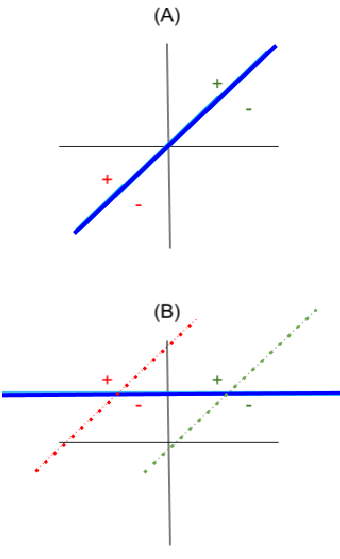
\includegraphics[width=60mm]{NegativeExample.png}
\caption{Example of incorrect monitoring by applying the LDA locally. The
initial state of the data is presented in (A) and the state at a later point
is shown in (B). In (B) every node (green and red dashed lines) calculates the same angle
for the separator as it was in (A). But it can be
seen that the true separator's (blue solid line) angle has changed
significantly.}
\label{NegativeExample}
\end{figure}


\par To overcome this difficulty, we turn to geometric monitoring. Geometric
monitoring \cite{keren2014geometric, keren2012shape} is a communication
efficient approach that monitors whether a function of distributed
data streams crosses a threshold. The key idea is to
impose constraints on local data at the nodes, rather than
on the function of the global aggregate. Given a function of
the average of all local data and the threshold, we compute a
``good'' convex subsets, called \textit{safe zones}, for each
node.

\par As we show below, convexity
plays a key role in the correctness of this scheme. As long
as local data stay inside the safe zones, we guarantee that
the function of the global average does not cross a threshold (given
in terms of maximal angle or norm of distance between the classifiers).
Nodes communicate only when local data drifts outside the
safe zone, which we call a safe zone \textit{violation} (hereafter,
violation). Once that happens, violations can be resolved, 
for example by aggregating data from all the nodes and recomputing $w_0$ 
and the safe zones.
In other words, we want to impose conditions on the local
data at each node so that as long as they hold, $||w-w_0||<R_0$.

\subsection{Notation}
\noindent
$P$ and $Q$ are the classes in the binary classification problem.
 $p,q,p^i$ and $q^i$  are the global and local means of classes $P$ and $Q$.
\\$S$ and $S^i$  are the global and local normalized scatter matrices of the feature space:
\\$S^i := \frac{1}{n}\sum_{j=1}^{n}x^i_j(x^i_j)^T
\\S := \frac{1}{nk}
\sum_{i=1}^k\sum_{j=1}^nx^i_j(x^i_j)^T=\frac{1}{k}\sum_{i=1}^kS^i$.
\\Similarly, $u$ and $u^i$ are the distance between the means of the classes:
\\$u:=p - q$
\\$u^i:=p^i - q^i$.
\\ $B$ is the global covariance matrix, which is the sum of the covariance
matrices of the two classes:
\\$B:=B_p+Bq$
\\It can be shown that
$B=S - pp^T - qq^T$.
%\\B^i:=S^i - p^i(p^i)^T - q^i(q^i)^T$
\\\\Let w be our current true model. Then, following Eq.~\ref{eq:w}, we can
express:
%\\$w(S,\mu_p,\mu_q) := (S - \mu_p\mu_p^T - \mu_q\mu_q^T)^{-1}(\mu_p - \mu_q)$
\begin{equation*}
w:=(S - pp^T - qq^T)^{-1}(p-q)=B^{-1}u.
\end{equation*}
%In the following the subscript $0$ will denote the state at the time 
%of last synchronization. 
Let $w_0$ be the existing model, previously computed from $(S_0, p_0, q_0)$
or from $(B_0,u_0)$ at the time of synchronization.
Then,
\begin{equation*}
w_0:=(S_0 - p_0p_0^T - q_0q_0^T)^{-1}(p_0-q_0)=B_0^{-1}u_0.
\end{equation*}
$\Delta_s, \delta_p$, and $\delta_q$ are the drift vectors of $S, p$, and $q$,
i.e.,
\begin{alignat*}{1}
& \Delta_s:= S - S_0 \\
& \delta_p:= p - p_0 \\
& \delta_q := q - q_0.
\end{alignat*}
\\If $S_0^i$, $p_0^i$ and $q_0^i$ are the local normalized scatter and averages
of the samples in a node, we can define the local drifts to be:
\begin{alignat*}{1}
& \Delta_s^i:= S^i - S_0^i
\\ & \delta_p^i:= p^i - p_0^i
\\ & \delta_q^i:= q^i - q_0^i.
\end{alignat*}
\begin{remark} \label{average}
It is easy to see that every global drift is the average of the local drifts:
\begin{alignat*}{1}
& \Delta_s = \frac{1}{k} \sum \Delta_s^i, \\
& \delta_p = \frac{1}{k} \sum \delta_p^i, \\
& \delta_q = \frac{1}{k} \sum \delta_q^i.
\end{alignat*}

\end{remark}

\subsection{Convex Safe Zones}
Each node monitors its own drift: as long as current values
at local nodes $(S^i,p^i,q^i)$ are sufficiently similar to their values
at synchronization time $(S^i_0,p^i_0,q^i_0)$, $w_0$ is guaranteed to be close to $w$.
Formally, we define a convex set $\mathcal{C}$ such that:
\begin{equation} \label{convex}
(\Delta_s, \delta_p, \delta_q) \in \mathcal{C} \Rightarrow \parallel w-w_0
\parallel \ < R_0.
\end{equation}
\begin{lemma}
Let $\mathcal{C}$ be a convex set that satisfies Eq. \ref{convex}.
If $(\Delta_s^i, \delta_p^i, \delta_q^i) \in \mathcal{C}$ for all i, then
\begin{equation*}
\parallel w-w_0 \parallel \ < R_0.
\end{equation*}
\end{lemma}
\begin{proof}
We express $S, p$ and $q$ as their values at synchronization with the addition of the
average of the local drifts:
\begin{equation*}
\begin{split}
(S,p,q) & = \frac{1}{k} \sum_i (S^i,p^i,q^j) \\
 & = (S_0,p_0,q_0) + \frac{1}{k} \sum_i (\Delta_s^i,\delta^i_p,\delta_q^i). \\
\end{split}
\end{equation*}
From $\mathcal{C}$'s convexity and using Remark \ref{average} we get:
\begin{equation*}
\begin{split}
\forall i (\Delta_s^i,\delta^i_p,\delta_q^i) \in \mathcal{C} & \Rightarrow
\frac{1}{k} \sum_i (\Delta_s^i,\delta^i_p,\delta_q^i) \in \mathcal{C} \\
& \Rightarrow (\Delta_s,\delta_p,\delta_q) \in \mathcal{C}.
\end{split}
\end{equation*}
Finally, from the definition of $\mathcal{C}$ we obtain:
\begin{equation*}
(\Delta_s,\delta_p,\delta_q) \in \mathcal{C} \Rightarrow \parallel w-w_0
\parallel \ < R_0,
\end{equation*}
\end{proof}

\subsection{Convex Bound For Local Condition}
We denote the drift in the global covariance matrix
\begin{alignat*}{2}
\Delta & := && B-B_0 \\
& = && (S_0+\Delta_S - (p_0+\delta_p)(p_0+\delta_p)^T \\
& && - (q_0+\delta_q)(q_0+\delta_q)^T) \\
& && - (S_0 - p_0p_0^T - q_0q_0^T) \\
& = && - \delta_p\delta_p^T - \delta_q\delta_q^T \\
& && + \Delta_S - p_0\delta_p^T \\
& && - \delta_pp_0^T - q_0\delta_q^T - \delta_qq_0^T.
\end{alignat*}
We break $\Delta$ into its quadratic part,
\begin{equation*}
M:= - \delta_p\delta_p^T - \delta_q\delta_q^T
\end{equation*}
\begin{equation*}
M^i:= - \delta_p^i(\delta_p^i)^T - \delta_q^i(\delta_q^i)^T
\end{equation*}
and its linear part,
\begin{equation*}
L:= \Delta_S - p_0\delta_p^T - \delta_pp_0^T - q_0\delta_q^T - \delta_qq_0^T
\end{equation*}
\begin{equation*}
\\ L^i := \Delta_S^i - p_0^i(\delta_p^i)^T - \delta_p^i(p_0^i)^T -
q_0^i(\delta_q^i)^T - \delta_q^i(q_0^i)^T,
\end{equation*}
and hence
\begin{equation*}
\Delta= L+ M.
\end{equation*}
We denote the drift of the distance between the means as
\begin{equation*}
\delta:= u-u_0 = \delta_p - \delta_q.
\end{equation*}
Now we can state a convex bound for our problem:
\begin{lemma} \label{convexBound}
If $\mathcal{G}$ is the set of triplets $(\Delta_s^i, \delta_p^i, \delta_q^i)$
 that satisfies the bound:
 \begin{equation} \label{eq:convexBound}
\begin{split}
||B_0^{-1}\delta|| &+ (||w_0||+R_0)(||B_0^{-1}L||+||B_0^{-1}M||) \\ & \leq  R_0,
\end{split}
\end{equation}
such that
 \begin{equation*}
||B_0^{-1}\Delta|| < 1
\end{equation*}
 (where $||A||$ is the operator norm of the matrix $A$,) then $\mathcal{G}\subseteq \mathcal{C}$ and $\mathcal{G}$ is convex.
\end{lemma}
The proof of lemma \ref{convexBound} is given in Appendix A.

\section{Method}
In the following, we present two frameworks for LDA model monitoring that use
the bound in Eq. \ref{eq:convexBound}. In both frameworks, every node runs the same
update algorithm as detailed in Alg. \ref{NodeUpdate}.
The frameworks differ in their synchronization policy. %violation recovery policy.
The first,Distributed LDA Monitoring (DLDA), will synchronize in a round
in which at least one node has reported a violation as detailed in Alg.
\ref{DLDA}).
The second, Probabilistic Distributed LDA Monitoring (PDLDA), will synchronize in
a round in which the number of nodes with violation is above a certain
threshold.
The derivation of this threshold is presented Section \ref{sec:PDLDA}.


\begin{algorithm}
\caption{Node Update: $i$ is the index of the node, $(x,y)$ is a new sample.}
\label{NodeUpdate}
\begin{algorithmic}[1]
\Procedure{Update}{}
\If {$y$ is class P}
\State $p^i = p^i + x - x_{old}^i(p)$
\State $S^i = S^i +xx^T - x_{old}^i(p)*(x_{old}^i(p))^T$
\Else
\State $q^i = q^i + x -x_{old}^i(q)$
\State $S^i = S^i +xx^T - x_{old}^i(q)*(x_{old}^i(q))^T$
\EndIf
\State $(\Delta_s^i,\delta^i_p,\delta_q^i) = (S^i-S^i_0,p^i-p^i_0,q^i-q^i_0)$
%\If{The bound in \ref{eq:convexBound} is not satisfied}

\If { \begin{varwidth}[t]{\linewidth}
$||B_0^{-1}\delta^i||+ (||w_0||+R_0)(||B_0^{-1}L^i||+||B_0^{-1}M^i||) $ \par
\hskip\algorithmicindent $>R_0$}
\end{varwidth}
\State Report violation to coordinator
\State Receive new global $B_0^{-1}$, $||w_0||$
\State $(S_0^i,p_0^i,q_0^i) = (S^i,p^i,q^i)$
\EndIf

\EndProcedure
\end{algorithmic}
\end{algorithm}

\begin{algorithm}
\caption{Coordinator violation resolution algorithm.}\label{DLDA}
\begin{algorithmic}[1]
\Procedure{Sync}{}
\If {One of the nodes has reported for violation}
\State Receive from every node $i$ the triplet $(S^i,p^i,q^i)$
\State Compute updated $||w_0||$ and $B_0^{-1}$ and distribute.
\EndIf
\EndProcedure
\end{algorithmic}
\end{algorithm}

\subsection{Probabilistic Distributed LDA Monitoring}\label{sec:PDLDA}

DLDA triggers synchronization when a single node reports violation.
Our empirical evaluation with a large number of nodes showed that such strict
policy causes synchronization when the global model is still valid. The likely
reason for this phenomenon is that theoretical bound is not tight enough. 
To resolve this problem we suggest to relax the synchronization policy of 
the system and synchronize when a certain portion of nodes report violation. 
Next, we derive a threshold on the number of nodes with violation that indicates 
that the change in the global model is higher than the permitted level. 
To compensate for relaxing the threshold on the number of violated nodes
(from 1), we lower the threshold on the model change $\|w-w_0\| \geq R_0$  
to $u<R_0$.

Let $U\in\{0,1\}$ be an indicator variable, such that $U=1$, 
when $\|w-w_0\| \geq u$ and $U=0$ otherwise (now, $U=1$ indicates the violation).
Let $v_i \in \{0,1\}$ be an indicator for a local violation in the
$i$'th node. We define the probability for True Positive (TP) and False Positive
(FP) in a node as:
\begin{alignat*}{1}
& P_{TP} := P(v_i=1 | U=1) \\
& P_{FP} := P(v_i=1 | U=0).
\end{alignat*}
Let $V$ be the random variable denoting the number of local violations
\begin{equation*}
V := \sum_{i=1}^k v_i.
\end{equation*}

We denote the minimal number of violations that causes a synchronization 
as a violation threshold $t$ and it is quantified by 
$t:=k*P_{FP}+z$ for some integer $z$.
We would like to derive a condition that for a given $0 < \epsilon < 0.5$ 
guarantees that
$P(V>t|U=0) < \epsilon$.
\\From the Chernoff bound it follows that
\begin{alignat*}{1}
& P(V>t | U=0) \\
& = P(V>k*P_{FP}+z | U=0) \\
& \leq \exp(-\frac{z^2}{2kP_{FP}(1-P_{FP})}) \\
& \leq \epsilon.
\end{alignat*}
For $z^*:=\sqrt{2kP_{FP}(P_{FP}-1)\log(\epsilon)}$ the condition is satisfied.
Consequently, for $t^*:=k*P_{FP}+z^*$,  $$P(V > t^*|U=0) <
\epsilon$$
We found a threshold $t^*$ on the number of nodes with violation, such that if $V > t^*$,  then
$\|w-w_0\| \geq u$ with high probability, and thus requires synchronization.
\section{Evaluation}
We evaluated the performance of the proposed monitoring algorithms,
DLDA and PDLDA, on synthetic and real
data. For each dataset we simulated a distributed data stream by partitioning the data between the nodes and streaming it one sample in a round. We defined a coordinator, whose role is to monitor the violation alerts from the nodes and aggregate the data from all the nodes when it happens. The coordinator recomputes the model after data aggregation and sends the new covariance matrix and the norm of the new model to the nodes (in privacy preserving mode, the coordinator is a trusted party).
%To analyse the performance of the methods, we counted the number of synchronizations and recorded the deviation between the true and the monitored models.

\subsection{Synthetic Data Experiments}
We use a synthetic data, in which all model assumptions hold, to
exemplify the communication efficiency of our method (Section \ref{sec:com_eff}) and the ability to detect a concept drift before the error occurs (Section \ref{sec:earlydetection}). We then (Section \ref{sec:paramanal}) analyse the communication efficiency of our method as a function of algorithm parameters.

\subsubsection{Communication Efficiency}\label{sec:com_eff}
We compare DLDA to the T-periodic algorithm, denoted
PER(P), which is a simple sampling algorithm that sends updates
every P rounds.
Our main performance metric is communication, measured
in \textbf{normalized messages} -- the average number of messages sent per
round by each node. PER can achieve an arbitrarily low communication at the price of errors. Periodic synchronization can miss the point of change in the data, hence it cannot guarantee to keep the model drift under a fixed threshold, while DLDA can.  DLDA has additional intrinsic advantages over PER: 1) DLDA can be instantly calibrated to fit a given drift threshold, while for PER the interval between synchronizations could only be determined empirically, which is slower. 2) Contrarily to PER, DLDA does not require adaptation period when the rate of the concept drift changes.
%1) For a given allowed error rate, DLDA can be immediately calibrated not to exceed it while for PER the right period has to be found empirically.
%2) If the rate that the date evolves changes, PER won't adapt its period size,
%while DLDA adapts immediately.
	
Figure \ref{PERvsDLDAoverTime} shows the behavior of the DLDA monitoring
algorithm over a synthetic dataset with 3 concept drifts.
DLDA achieves communication of 0.01 messages per node per round, and
the model drift is always below the given threshold.
Conversely, the equivalent PER(100) algorithm doesn't maintain the
model drift below the threshold.
Figure \ref{PERvsDLDAoverTime} shows that the periodic algorithm does not always  synchronize when the model drift exceeds a given threshold. Moreover, it  triggers redundant synchronization when there is no concept drift.

\subsubsection{Early Drift Detection}\label{sec:earlydetection}
Consider a toy example (see Figure \ref{EarlyDetection}), in which a 2D data arrives from two classes (the positive class is represented by circles and the negative by asterisks), each one following a 2D arc in the opposite direction. The class is switched at each round. Both classes have a drift towards the separation boundary, which eventually crosses it, causing the classification error (at time $t_last$). We apply DLDA method to detect violation, and it detects it prior to the time  (with some margin) when the misclassification occurs (see the point of violation alert in figure \ref{EarlyDetection}). This example demonstrates an important advantage of our method over error-based concept drift methods, that detect drift only after the model becomes inaccurate or invalid.

\subsubsection{Parameter Analyses}\label{sec:paramanal}
Next, we analyse the parameters of the DLDA algorithm. 

\noindent\textbf{Drift Threshold:} Figure \ref{PERvsDLDAoverError} shows the communication requirements of the DLDA algorithm as a function of the model drift threshold, and the minimal communication required to match DLDA using the PER.	
It can been seen that for both fixed and dynamic data, DLDA outperforms PER for
any given drift threshold.
 \begin{figure}[ht]
	\centering
	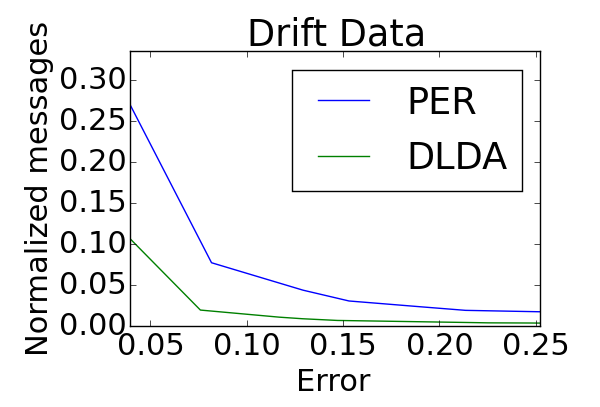
\includegraphics[width=60mm]{PER/onlyDrift.png}
	\caption{Communication as the function of drift for DLDA and PER. The
	periodic algorithm is tuned to achieve the same max drift as DLDA
	for each threshold.}
	\label{PERvsDLDAoverError}
	\end{figure}

	
\noindent\textbf{Node Scalability:}
Figure \ref{Nodes} shows the communication volume as a function of the number of nodes $k$.
We observe that communication increases slowly, reaching 0.25\% on the fixed
data and 0.6\% on the dynamic data distributed across 25 nodes.
	\begin{figure}[h]
	\centering
	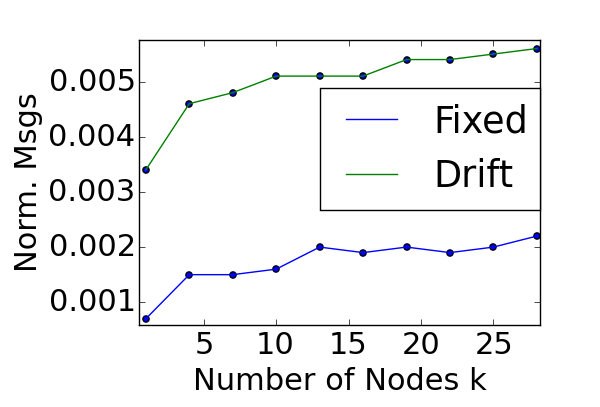
\includegraphics[width=60mm]{CommunicationOfFixedVsDrift/Nodes.png}
	\caption{Communication as a function of the number of nodes.}
	\label{Nodes}
	\end{figure}
%\subsubsection{Dimension}
%Figure \ref{Dimension} shows how the dimension of the dataset affects
%communication.
%When window size $W$ is fixed, communication grows linearly with dimension $d$.
%	\begin{figure}[h]
%	\centering
%	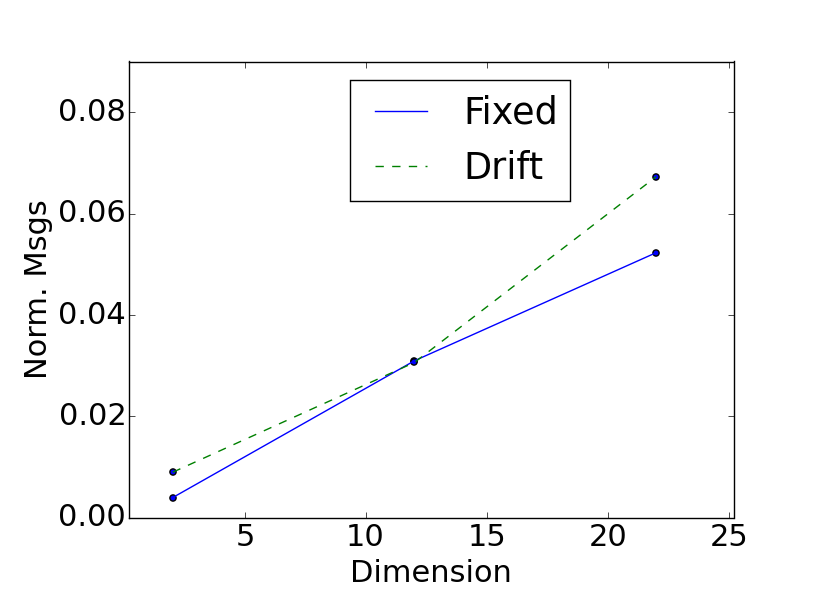
\includegraphics[width=60mm]{CommunicationOfFixedVsDrift/Dimension.png}
%	\caption{Communication as a function of input dimension}
%	\label{Dimension}
%	\end{figure}

\noindent\textbf{Window Size:}
Figure \ref{WindowSize} shows how communication decreases as a result
of enlarging the window size $W$.  One can increase the window size to compensate for other factors in the system that increase the communication. One of those is
noise (which is quantified in our context by the standard deviation of the
data generating distribution).
 \begin{figure}
	\centering
	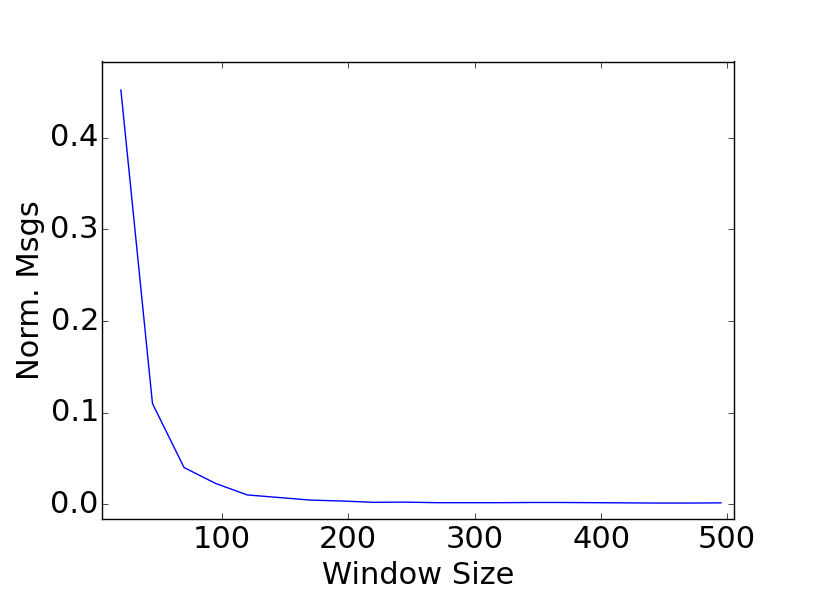
\includegraphics[width=60mm]{CommunicationOfFixedVsDrift/WindowSize.png}
	\caption{Communication as function of window size $W$}
	\label{WindowSize}
	\end{figure}
%\subsubsection{Noise}
Figure \ref{Noise} shows normalized messages obtained for different
noise magnitudes. The experiment shows that the drift grows with the noise, causing more synchronizations (more communication). This is result is not surprising, and the solution for it is increasing the window size. 

Another parameter that is directly related to the window size is the dimension of the data. The number of samples required for accurate estimation of the covariance matrix grows with the dimension. In our settings, the number of training samples is linked to the window size. When window size is fixed, communication grows linearly with the dimension (see Figure \ref{Dimension}).
	
\begin{figure}
	\centering
	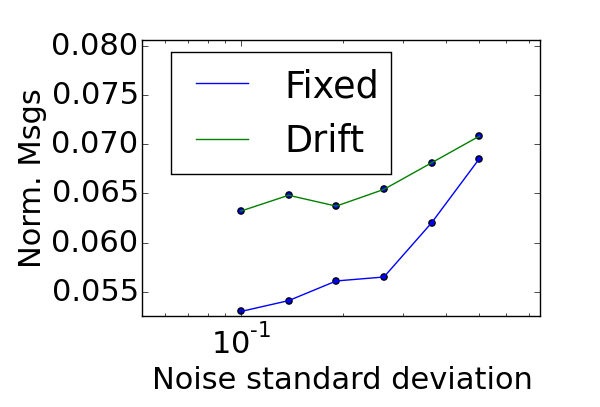
\includegraphics[width=60mm]{CommunicationOfFixedVsDrift/Noise.png}
	\caption{Communication as a function of the standard deviation of the
	data generating distribution.}
	\label{Noise}
	\end{figure}

\begin{figure}
	\centering
	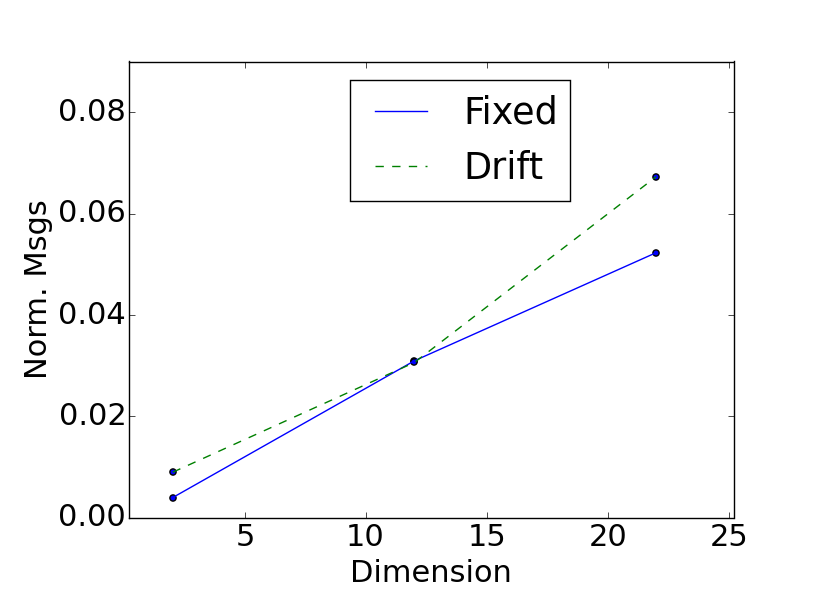
\includegraphics[width=60mm]{CommunicationOfFixedVsDrift/Dimension.png}
	\caption{Communication as a function of input dimension}
	\label{Dimension}
	\end{figure}

\subsection{Real Data Experiments}
In this section we demonstrate the algorithm with 3 datasets. The first
(newsgroups collection) is relatively small, small enough for using
the deterministic DLDA algorithm and there is no need to use PDLDA.
The second (Power Consumption Monitoring) is a medium size dataset (it
is distributed over 36 nodes) and both DLDA and PDLDA are demonstrated on it.
The third (Gas Sensor Time Series Monitoring) is big (it is distributed over
100 nodes), so we had to use only PDLDA on in.
\subsubsection{Message Preference Monitoring --- Usenet}
The USENET dataset is described in \cite{usenet}.
This is a text dataset that simulates a stream of messages from three newsgroups
(medicine, space, baseball); the messages are presented sequentially to a user,
who then labels them as interesting or junk, according to personal interest.
Attribute values are binary, indicating the presence or absence of the 128
informative words. The drift occurs from an artificial change in the user's
preference (from space to baseball). In Figure \ref{usenet} the behavior of the
DLDA algorithm with $W=450$ is presented. The first 450 rounds over the data are for
initialization and are omitted. During the next 50 rounds the DLDA error
(the value is calculated on the left side of inequality
\ref{eq:convexBound}) increases due to noise in the data; there is
no concept drift. From round 500 to 600 the DLDA error is stable,
and again is due only to the noise. In round 600 there is a concept
drift.
From this point both the DLDA and the true error increase until the
synchronization in round 698.

\begin{figure}[h]
	\centering
	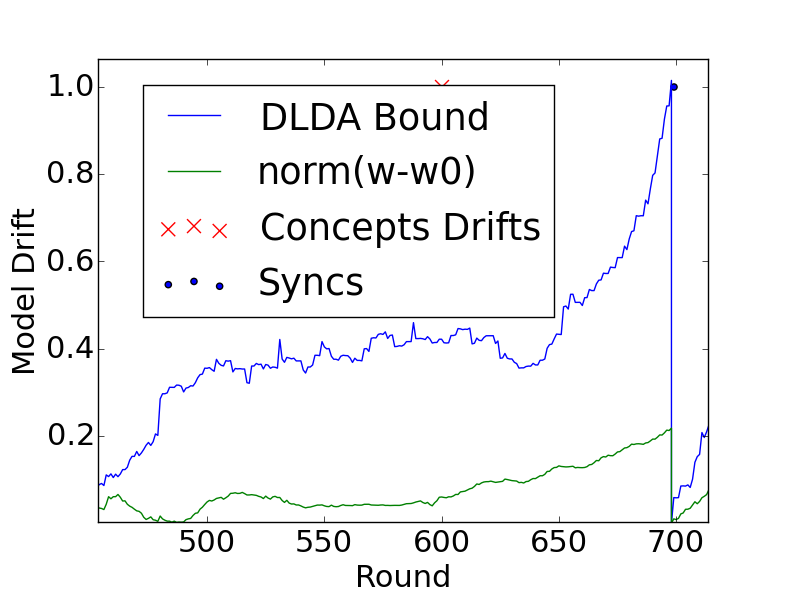
\includegraphics[width=60mm]{Usenet/DriftDetected.png}
	\caption{Comparison between maximal (over nodes) DLDA (blue)
	error and the true global error (green) for $k=2$, $W=450$.
	It can be seen that DLDA responds to the concept drift that occurs
	after 600 rounds (red x) and causes a synchronization in round 698 (blue dot).}
	\label{usenet}
	\end{figure}
	
\subsubsection{Power Consumption Monitoring}
The Power Consumption dataset contains the hourly power supply of an
Italian electric company as recorded from two sources: power supplied
by the main grid and power transformed from other grids.
This stream contains three-year power supply records
from 1995 to 1998, and our learning task is to predict which hour (1 out of 24 hours) the
current power supply belongs to. The concept drift in this stream
is mainly driven by factors such as the season, weather, time of day,
and the differences between working days and weekend.
The dataset is described and can be downloaded from \cite{powerSupply}.
We demonstrate the algorithms on the following binary classification problem:
given a power supply measurement, decide if it is a night or a day.
This dataset is an example of gradual concept drift (seasons do not
change suddenly).
In Figure \ref{PowerSupplyFigures} DLDA
and PDLDA are demonstrated. For a small number of nodes, $k=4$, and for big
window size, $W=5000$, the communication is reduced to 0.3\%.
For a more distributed system, k=36, and a smaller window
size, $W=600$, the communication is reduced to 9\%. For PDLDA with
$k=36$ and $W=600$ and a violation threshold (VT) of 50\%, the communication
is reduced to 2\%.





\begin{figure}
    \centering
    \begin{subfigure}[b]{0.5\textwidth}
        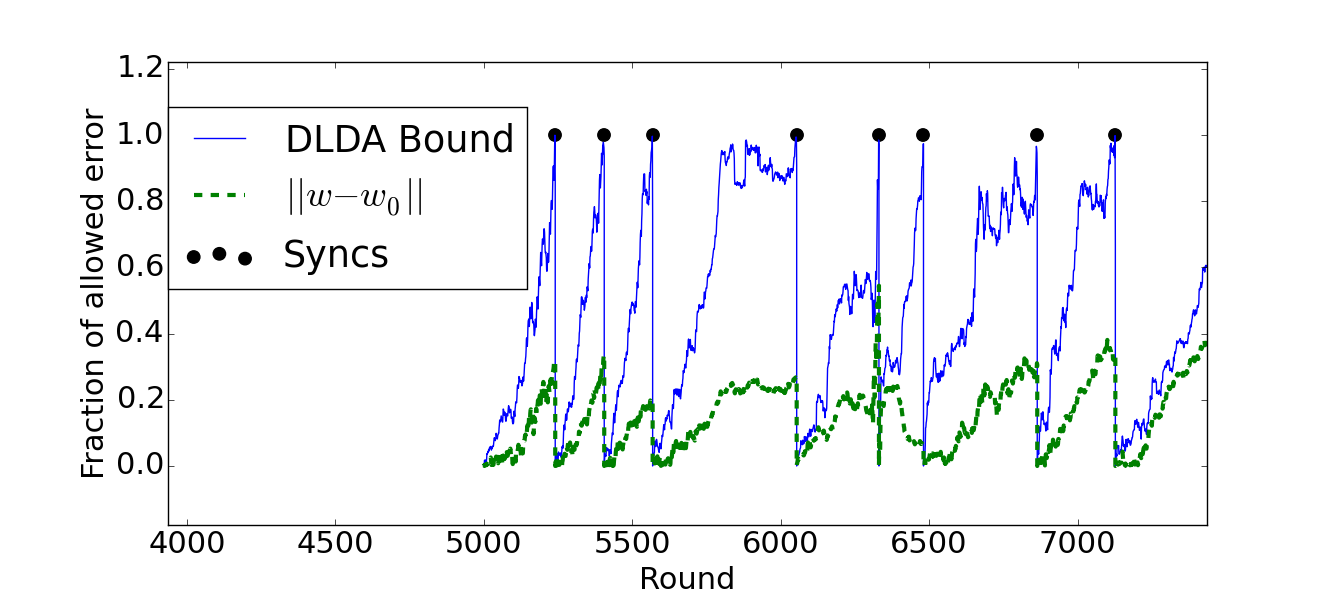
\includegraphics[width=\textwidth]{PowerSupply/4nodes.png}
        \caption{k=4, W=5000, VT=0}
        \label{fig:gull}
    \end{subfigure}

    \begin{subfigure}[b]{0.5\textwidth}
        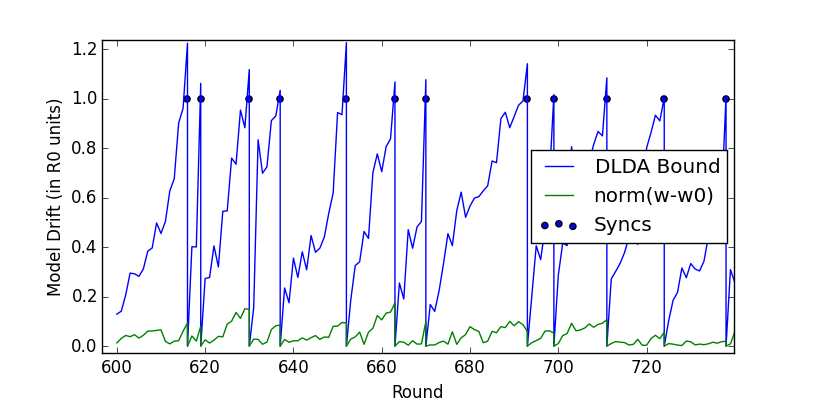
\includegraphics[width=\textwidth]{PowerSupply/36nodes.png}
        \caption{k=36 Nodes, W=600, VT=0}
        \label{fig:tiger}
    \end{subfigure}

    \begin{subfigure}[b]{0.5\textwidth}
        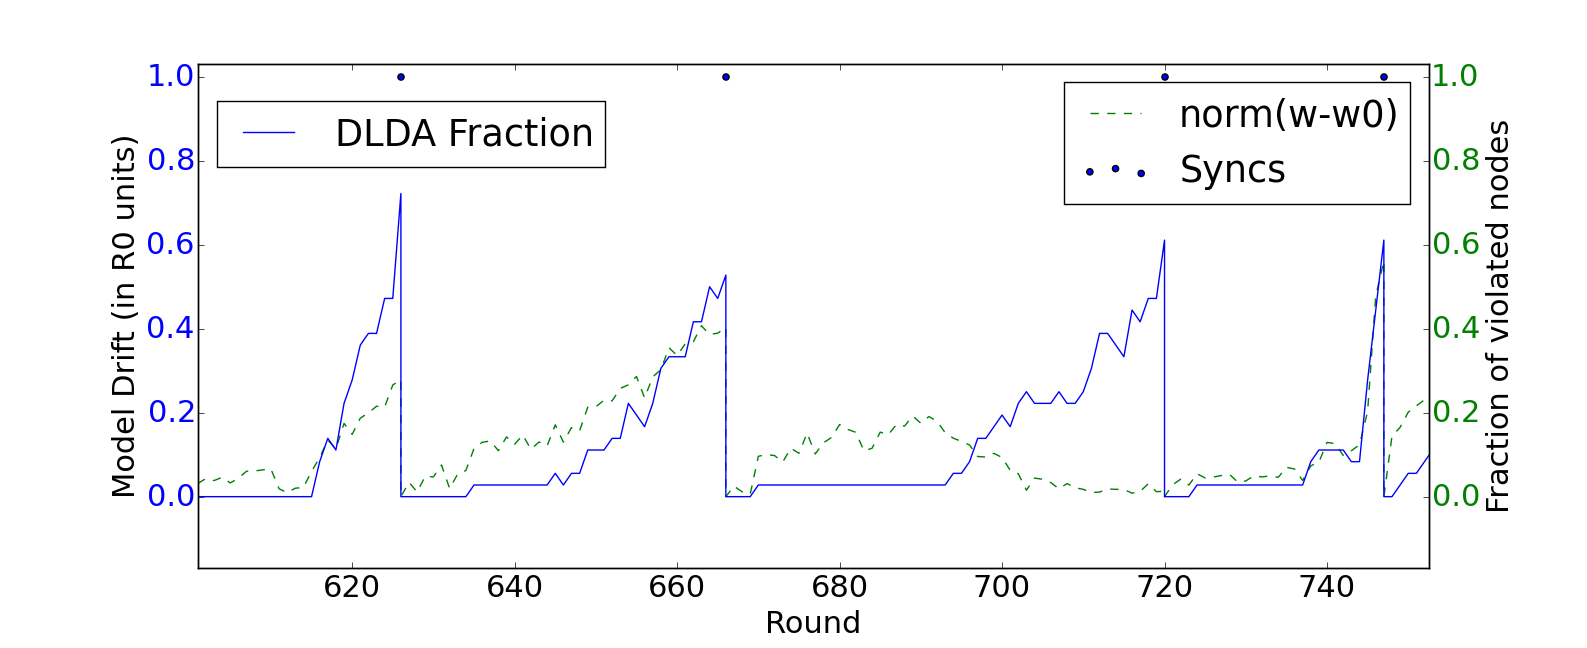
\includegraphics[width=\textwidth]{PowerSupply/36nodesProb.png}
        \caption{k=36 Nodes, W=600, VT=0}
        \label{fig:mouse}
    \end{subfigure}
    \caption{In the first two figures the DLDA algorithm adapts
  to gradual concept drift on the power supply dataset.
  The maximal error (over the nodes) in the
  local DLDA bound calculation (blue) is compared to the true
error (the norm of the difference) of all the data aggregated from
all of the nodes (green). In the last figure PDLDA
is demonstrated on the same dataset; the blue curve represents the
fraction of violated nodes.}\label{PowerSupplyFigures}
\end{figure}




\subsubsection{Gas Sensor Time Series Monitoring}

\begin{figure}[h!]
\centering
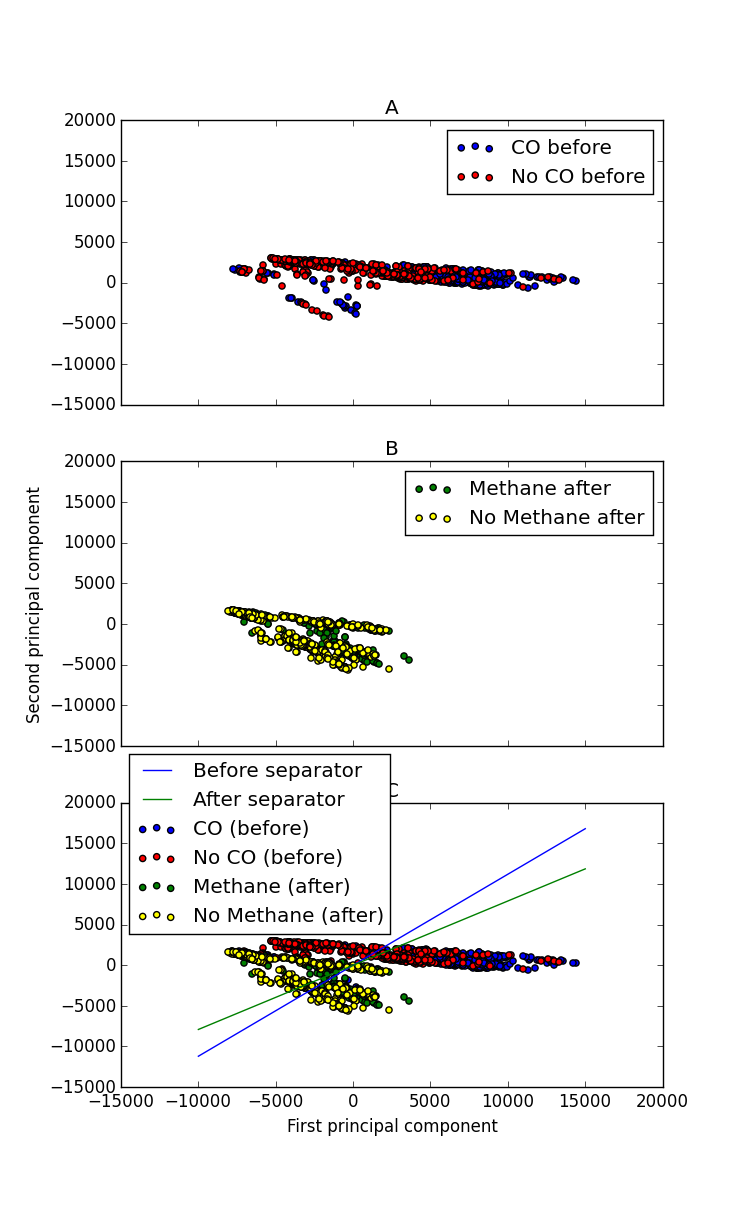
\includegraphics[width=60mm]{BigGas/showData.png}
\caption{Two-dimensional PCA projection of the gas sensor data,
before concept drift (A), after concept drift (B),
and the two projections together with their separators (C).
The plot comes to illustrate the true change in the classifiers angle (as PDLDA
behaviour indicates).}
\label{BigGasShowData}
\end{figure}


\begin{figure*}[ht!]
\centering
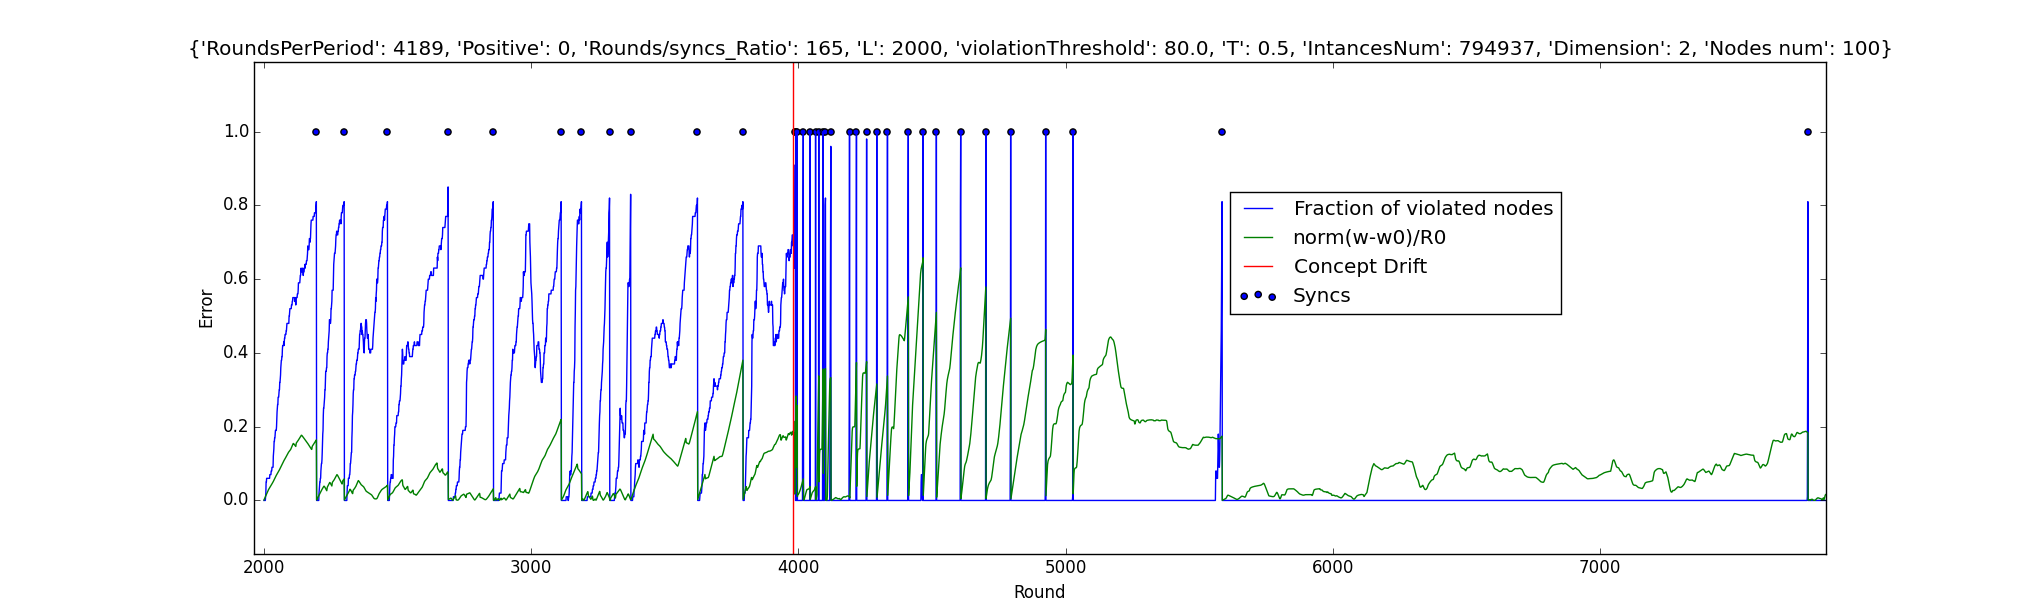
\includegraphics[width=\textwidth]{BigGas/overTime100k.png}
\caption{Demonstration of PDLDA on the Gas Sensor dataset.
A comparison between the true error (green) to the fraction of the nodes that
are violated in the current round (blue).
The experiment is configured for k=100 nodes, and the violation threshold is
VT=80.}
\label{BigGasOverTime}
\end{figure*}
Data in this experiment \cite{bigGas} consists of measurements collected
by an array of 16 chemical sensors in a lab, recording at a sampling
rate of 100Hz for 24 hours, resulting in 8378504 data points for each sensor.
During the first 12 hours the task is to detect the presence of carbon monoxide
(CO) in a mixture of Gases, and from the 13th hour the task is to detect the presence of methane.
The change between the first task to the second is the sudden concept drift.
In Fig \ref{BigGasShowData} a PCA projection of the data is shown.
This is a big dataset, and can be massively distributed.
There are two kinds of drifts in the data: there is a gradual drift that comes from
the change in temperature in the lab over time, and an
artificial sudden drift that comes from the switch between tasks after 12 hours.
Figure \ref{BigGasOverTime} demonstrate the results of PDLDA.

In Figure \ref{BigGasOverTime} two phenomena can be observed.
First, the two lines are highly correlated --- the fraction of the violated
nodes follows the true error. Second,  before the sudden concept drift
(marked by the vertical red line), there is a synchronization every 150 rounds, while
after the concept drift there is a synchronization only every 50 rounds.
The second phenomenon continues over 1000 rounds, where there is a mixture in the
sliding window between old (before the concept drift) data and new
(after the concept drift). The existence of the second phenomena shows that
the PDLDA algorithm detects and responds to the sudden concept drift.


\section*{Conclusions}
We introduced a first communication-efficient monitoring algorithm for a linear classifier model that monitors the
models itself, but doesn't need the knowledge of the global model at local nodes.
As long as all nodes meet their local condition, the
global model is guaranteed to be valid. Our algorithm has important benefits:
\begin{itemize}
  \item Our method works with the distributed data in communication efficient way.
  \item Monitoring the model as oppose to errors allows for early detection of the drift before the violation of the model occurs.
  \item Our algorithm is privacy aware in the sense that it preserves privacy of the data at each node from other nodes.
\end{itemize}

We evaluated the theoretical scheme -- DLDA  and its probabilistic version --PDLDA, on three real data sets.
For a small number of nodes we used DLDA with its theoretical guarantee, and for a greater number of nodes we used
PDLDA and we showed that the proposed scheme outperforms PER: it maintains a smaller Euclidean distance between
the last computed model to the current true model with a lower volume of communication.

This work is the first step in designing communication-efficient algorithms with theoretical guarantees for monitoring classification models over dynamic streaming distributed data. Since we link the monitoring algorithm with the hypothesis class and the learning algorithm, each classifier type should be studied in depth. Alternatively, one can think of developing a monitoring method for a given hypothesis class, independent of the training algorithm. One of the future directions is to extend the proposed framework to ensemble of linear classifiers and neural networks, including deep learning network.
An orthogonal, but important research direction is to analyse the privacy aspect of the proposed algorithm and try to adjust the proposed scheme  in order to provide a better privacy of the local data.

%
% The following two commands are all you need in the
% initial runs of your .tex file to
% produce the bibliography for the citations in your paper.
\bibliographystyle{abbrv}
\bibliography{bib}  % sigproc.bib is the name of the Bibliography in this case
% You must have a proper ".bib" file
%  and remember to run:
% latex bibtex latex latex
% to resolve all references
%
% ACM needs 'a single self-contained file'!
%

\appendix
\section{Appendix} \label{AppendixA}
To find a convex subset C satisfying the condition of Eq. \ref{convex},
We first define the operator norm:
\begin{definition}
Let $A$ be a matrix. Its operator norm, or
spectral norm, hereafter just norm, is defined as:
\begin{equation*}
||A|| = \sup_{x \neq 0}\frac{||Ax||}{||x||}.
\end{equation*}
\end{definition}

\begin{lemma} \label{lemma:newman}
If A is square and $||A|| < 1$, then
\begin{equation*}
||(I+A)^{-1}|| < \frac{1}{1-||A||}.
\end{equation*}
\end{lemma}
The proof for this lemma can be found in \cite{gabel2015monitoring}.

\subsection{Convex Bound Proof}
We recall that $\mathcal{C}$ is the convex subset that satisfies
inequality \ref{convex} and $\mathcal{G}$ is the set of triplets
$(\Delta_s^i, \delta_p^i, \delta_q^i)$
 that satisfies the inequality \ref{eq:convexBound}.

\begin{lemma}
$\mathcal{G} \subseteq \mathcal{C}$:
\end{lemma}

\begin{proof}
We can write the sphere condition in terms of $B_0, \Delta, u_0$ and $\delta$ using the triangle
inequality:
\begin{equation} \label{in}
\begin{split}
||w-w_0|| & = \ ||(B_0+\Delta)^{-1}(u_0+\delta) - B_0^{-1}u_0|| \\
& < ||(B_0+\Delta)^{-1}\delta|| \\
& \ \ + ||((B_0+\Delta)^{-1} - B_0^{-1})u_0||.
\end{split}
\end{equation}

We split the right side of the last inequality into two parts:
\begin{equation}  \label{e1e2}
\begin{split}
& E_1:= ||(B_0+\Delta)^{-1}\delta|| \\
& E_2:= ||((B_0+\Delta)^{-1} - B_0^{-1})u_0||.
\end{split}
\end{equation}
Under the assumption of $||B_0^{-1}\Delta||\ \leq \ 1$,
it follows from lemma \ref{lemma:newman}:
\begin{equation} \label{e1e2In}
\begin{split}
& E_1 \leq \frac{||B_0^{-1}\delta||}{1-||B_0^{-1}\Delta||} \\
& E_2 \leq  \frac{|| B_0^{-1}\Delta w_0||}{1-||B_0^{-1}\Delta||}.
\end{split}
\end{equation}
From the Cauchy-Schwarz inequality we get:
\begin{equation} \label{CS}
||B_0^{-1}\Delta w_0|| \ \leq \ ||B_0^{-1}\Delta||||w_0||.
\end{equation}
Substituting Eq. \ref{e1e2}, \ref{e1e2In} and \ref{CS} in Eq. \ref{in}, we
get:
\begin{equation}
\begin{split}
|| w-w_0 \parallel & \leq \ E_1+E_2 \\
& \leq \frac{||B_0^{-1}\delta|| + ||B_0^{-1}\Delta||||w_0||}{1 -||B_0^{-1}\Delta||} \\
& \leq R_0.
\end{split}
\end{equation}
After rearranging the terms, we get
\begin{equation} \label{lostDenom}
||B_0^{-1}\delta|| + ||B_0^{-1}\Delta||||w_0||.
\leq R_0(1 -||B_0^{-1}\Delta||)
\end{equation}
From the triangle inequality we can rewrite:
\begin{equation} \label{linQuad}
||B_0^{-1}\Delta|| \leq ||B_0^{-1}L||+||B_0^{-1}M||.
\end{equation}
And finally, combining inequalities \ref{lostDenom} and \ref{linQuad},
we get the following bound:
\begin{alignat*}{2} \label{convexBound}
&||B_0^{-1}\delta|| &+ (||w_0||+R_0)(||B_0^{-1}L||+||B_0^{-1}M||)  \\
& \leq R_0.
\end{alignat*}
\end{proof}

\begin{lemma} \label{delta}
$||B_0^{-1}\delta||$ is convex in $\delta$.
\end{lemma}
\begin{proof}
Multiplication by $B_0^{-1}$ is a linear operation and norm is convex
operation. Therefore $||B_0^{-1}\delta||$ is convex in $\delta$.
\end{proof}

We recall that:
\begin{equation*}
L:= \Delta_S - p_0\delta_p^T - \delta_pp_0^T - q_0\delta_q^T - \delta_qq_0^T.
\end{equation*}
\begin{lemma} \label{L}
$||B_0^{-1}L||$ is convex in $\Delta_s, \delta_p$
and $\delta_q$.
\end{lemma}
\begin{proof}
$L$ is linear in the variables and therefore convex in these variables.

\end{proof}

We recall that:
\begin{equation*}
M:= - \delta_p\delta_p^T - \delta_q\delta_q^T.
\end{equation*}

\begin{lemma} \label{M}
$||B_0^{-1}M||$ is convex in $\delta_p$
and $\delta_q$.
\end{lemma}
\begin{proof}
From the definition of operator norm, we can rewrite the function as:
\begin{alignat*} {2}
||M|| & = && ||B_0^{-1}(\max_{||u||=1}{\{u^T \delta_p\delta_p^T u\}} +
\max_{||u||=1}{\{u^T \delta_q\delta_q^T u\}})||\\
& = && ||B_0^{-1}(\max_{||u||=1}{\{||u^T \delta_p||^2\}} +
\max_{||u||=1}{\{||u^T \delta_q||^2\}})||.
\end{alignat*}
We observe that max over a finite number of convex functions is also a convex
function, multiplication by a matrix and the norm keeps it convex.
This concludes our proof.
\end{proof}

\begin{corollary}
From lemmas \ref{delta}, \ref{L} and \ref{M} we can conclude that $\mathcal{G}$
is convex.
\end{corollary}
\end{document}

